\title{Организация\\
mark-and-sweep-сборщика мусора\\
в инфраструктуре LLVM}
%
\titlerunning{Организация mark-and-sweep сборщика мусора}
\author{Самофалов Александр Владимирович}
%
\authorrunning{А.В.Самофалов} % abbreviated author list (for running head)
%

% abbreviated author list (for running head)
%
%%%% list of authors for the TOC (use if author list has to be modified)
\tocauthor{А.В.Самофалов}
%
\institute{Санкт-Петербургский государственный университет\\
\email{aleksander.samofalov@gmail.com}}

\maketitle              % typeset the title of the contribution

\begin{abstract}
В данной работе описана реализация подключаемого модуля, который связывает между собой сборщик мусора и к
омпиляторную инфраструктуру LLVM. Также в работе описаны алгоритм сборки мусора mark-and-sweep, устройство 
дружелюбной к сборке мусора кучи и архитектура LLVM с точки зрения сборщика мусора.
\end{abstract}
%

\section*{Введение}
Задача построения эффективных и надежных компиляторов до сих пор является актуальной. Написать полностью собственный компилятор очень тяжело. Между тем при реализации компиляторов многие компоненты можно переиспользовать: для компиляторов для одного языка можно переиспользовать синтаксический анализатор, а для компиляторов в одну и ту же платфоррму -- генератор кода. Поэтому создаются специальные инфраструктуры разработки компиляторов, представляющие собой наборы средств, упрощающих разработку компилятора: переиспользуемых компонент, утилит, библиотек.

Одной из таких инфраструктур является Low Level Virtual Machine (LLVM)~\cite{llvm}. LLVM -- это набор иструментов и библиотек для анализа, трансформации и оптимизации программ. Она содержит в себе виртуальную машину для LLVM IR -- строго типизированного ассемблера, -- а также набор классов, позволяющих реализовать парсер и кодогенератор в этот язык. В настоящее время LLVM очень популярна, она используется многими крупными компаниями, такими как Apple и Intel. На основе LLVM написаны многие продукты, например, Clang~\cite{clang} -- известный компилятор для C и C++.

Память является одним из критических ресурсов приложения, поэтому важно правильно ею распоряжаться. 
Самым простым, эффективным и предсказуемым из всех способов управления памятью является ручное управление. 
Однако это не всегда возможно. Например, в функциональных языках программирования невозможно точно
определить время жизни объекта. Также ручное управление памяти требует от программиста внимательно следить
за освобождением каждого объекта, чтобы избежать утечек памяти -- возникновения областей, на которых нет ни одной 
хранящей их адрес ссылки.

С некоторыми проблемами ручного управления памятью позволяет бороться сборка мусора. 
Сборка мусора является одним из способов автоматического управления памятью. Сборщик мусора обходит участки памяти, определяя, 
какие из них недоступны из программы, и освобождает их. Существует много языков, в которых сборка мусора является обязательной,
например, Java, C\#, OCaml. 

Сборка мусора является частью среды времени исполнения и требует поддержки компилятора для корректной работы, а инфраструктура построения компиляторов должна обеспечивать взаимосвязь между ними. Также хочется иметь возможность переиспользовать написанный сборщик мусора при реализации другого языка программирования со сборкой мусора. Поэтому в инфраструктуре LLVM  существует возможность использовать подключаемые модули, отвечающие за взаимодействие среды времени исполнения и компилятора. 

Целью данной работы является реализация подключаемого модуля для компилятора LLVM, обеспечивающий взаимосвязь между 
сбощиком мусора и компилятором языка на основе LLVM.
Данная работа выполнена в рамках проекта лаборатории языковых инструментов компании JetBrains.

\section{Mark-and-sweep сборщик мусора}
Mark-and-sweep является самым старым алгоритмом сборки мусора: впервые он был описан в~\cite{lisp} и использован для сборки мусора в языке LISP. 
Алгоритм состоит из двух фаз. В первой фазе сборщик мусора находит и помечает все достижимые объекты. Объект называется достижимым, если на него указывает поле какого-нибудь другого достижимого объекта. Объекты, к которым программа может обратиться напрямую, называются корнями. Корни -- это локальные переменные на стеке или глобальные переменные, указывающие на объекты в куче. Корни считаются всегда достижимыми, поэтому для построения множества всех достижимых объектов достаточно найти все достижимые от корней обьекты. Это можно сделать, используя поиск в глубину. Для того, чтобы отличать достижимые обьекты от остальных, у каждого обьекта в куче должен быть выделен бит, который отражает это свойство.

Во второй фазе сборщик мусора обходит все объекты в куче и освобождает те из них, которые не помечены как достижимые. Для корректной работы при следующих сборках алгоритм также обнуляет все пометки о достижимости. 

Алгоритм целиком может быть описан следующим псевдокодом: 
\begin{algorithm}
\begin{algorithmic}[1]

\Function{gc}{}
  \ForAll{root $r$}
    \State \Call{mark}{$r$}
  \EndFor
  \State \Call{sweep}{}
\EndFunction

\Function{mark}{$q$}
  \If{$q$ is marked}
    \State \Return
  \EndIf
  \State {mark $q$}
  \ForAll{$p$ referenced by $q$}
    \State \Call{mark}{$p$}
  \EndFor
\EndFunction

\Function{sweep}{}
  \ForAll{$q$ in heap}
    \If {$q$ is not marked}
        \State {free $q$}
    \Else
        \State unmark $q$
    \EndIf
  \EndFor
\EndFunction

\end{algorithmic}
\caption{Mark-and-sweep}
\end{algorithm}

Недостатком mark-and-sweep является то, что для сборки мусора необходимо приостановить работу всей программы, что может быть неприемлемо для интерактивных программ или систем реального времени. Также во время сборки живые объекты не перемещаются, что может увеличить фрагментацию в куче, из-за которой может вырасти количество вызовов сборщика. 

Для реализации mark-and-sweep сборщика необходимы:
\begin{itemize}
  \item реализация кучи с поддержкой бита для пометки о достижимости, которая позволяет обойти все объекты;
  \item компилятор, который генерирует код и метаинформацию, позволяющие обойти все корневое множество;
  \item формат объектов, который позволяет определить, какие из полей являются указателями на объекты в куче.
\end{itemize}

\section{Обзор инфраструктуры LLVM}
Для того, чтобы реализовать компилятор на основе LLVM, достаточно написать транслятор в LLVM IR. Для генерации машинного кода LLVM есть кодогенератор для широкого набора современных платформ (x86, ARM, SPARC и другие). В состав LLVM входит модульный оптимизатор IR-кода. Каждая оптимизация являтся одним или несколькими проходами, которые можно отключать или подключать. Каждый проход может трансформировать или единицу трансляции целиком, или же содержимое функций. Желающему реализовать некоторую оптимизацию разработчику достаточно написать подключаемый модуль, в котором реализован проход, делающий эту оптимизацию. 

Поддержка сборки мусора в LLVM также представляется как содержащий несколько проходов подключаемый модуль. Чтобы сборщик мусора мог корректно определить, какие объекты являются живыми, а какие мусором, ему нужно обойти граф объектов. Для этого ему необходимо определить корневое множество -- указатели в стеке, регистрах и глобальной области памяти, которые ссылаются на объекты в куче. Такую возможность предоставляет встроенная в LLVM IR функция llvm.gcroot. Она принимает ссылку на указывающую на обьект в куче область памяти в стеке и указатель на метаданные. С помощью этой функции компилятор может отметить, какие обьекты на стеке являются корнями. LLVM сохраняет эту информацию для каждой функции, и позднее кодогенератор может ее использовать.

Некоторым сборщикам мусора может потребоваться информировать их о чтении или записи в поле находящегося в куче обьекта. Для этого  существуют механизмы барьеров чтения и записи, и LLVM предоставляет возможнось их использовать. Функции llvm.gcread и llvm.gcwrite реализуют эту возможность. Компилятор должен их использовать вместо load и store соответственно. Во время кодогенерации LLVM предоставляет подключаемому модулю возможность заменить вхождения этих функций на код барьера.

В подключаемом модуле можно указать необходимые для корректной работы сборщика мусора безопасные точки -- места в функциях, внутри которых безопасно запускать сборку мусора. LLVM предоставляет четыре типа безопасных точек:
\begin{itemize}
\item
  в конце итерации цикла;
\item
  во время выхода из функции инструкцией return;
\item
  до вызова функции;
\item
  после вызова функции.
\end{itemize}
LLVM сгенерирует структуру, в которую запишет все безопасные точки в каждой функции. Эту структуру позже может использовать кодогенератор.

Кроме трансформаций на уровне IR, LLVM предоставляет возможность записать нужную для сборки мусора информацию в начало или конец обьектного модуля.

LLVM позволяет легко переключаться от одного сборщика мусора к другому, достаточно лишь подключить другой подключаемый модуль. Более того, можно для каждой функции указать, какой модуль будет обрабатывать метаинформацию для нее. Для этого используется атрибут функции gc. 

\section{Описание реализации}
Для поддержки mark-and-sweep сборщика мусора реализован подключаемый модуль для LLVM. Модуль состоит из двух частей: трансформатора IR-кода и генератора метаинформации. Также была модифицирована куча для поддержки необходимой информации об объектах. Далее описана реализация каждого компонента.
\subsection{Транформатор IR-кода}
Транформатор IR-кода содержит два прохода: проход по единице трансляции и проход по функциям, для которых указано, что их должен обработать этот подключаемый модуль. Трансформатор кода обеспечивает доступность карты стека для каждой функции во время исполения, для этого он строит подобие цепочки вызова. В кадре стека функции сохраняется стукрура $StackChain$, в которой хранится указатель на карту стека для текущей функции и указатель на $StackChain$ для функции, вызвавшей ее. Указатель на последний $StackChain$ в этом списке записывается в глобальную переменную $chainBottom$. В итоге на стеке образуется односвязный список указателей на карты стека, с помощью которых сборщик мусора может определить корневое множество.
Для этого подключаемый модуль генерирует в прологе функции следующий код:

\begin{algorithm}
\begin{algorithmic}[1]
\State $currentChain \gets alloca~size(StackChain)$
\State $currentChain.meta \gets metadata for function$
\State $currentChain.prev \gets chainBottom$
\State $chainBottom \gets currentChain$
\end{algorithmic}
\caption{Пролог функции}
\end{algorithm}

На выходе из функции необходимо восстановить цепочку, которая была до вызова текущей функции. Для этого трансформатор кода ищет все инструкции ret и перед ними вставляет код, который меняет currentChain на правильный:

\begin{algorithm}
\begin{algorithmic}[1]
\State $chainBottom \gets currentChain.prev$
\end{algorithmic}
\caption{Эпилог функции}
\end{algorithm}

В LLVM существует поддержка механизма обработки исключений. Для этого используется инструкция invoke, которая принимает две метки: метку на участок кода, который должен выполниться после нормальной работы вызываемой фунцкии, и метку на участок кода с обработчиком ошибок. Управление переходит к обработчику ошибок, если вызываемая функция (или любая вызываемая в процессе функция) завершит работу с помощью оператора resume. Т.к. в результате этого управление может вернуться на несколько функций назад, то необходимо правильно обрабатывать эту ситуацию. Для этого трансформатор кода находит все вызовы invoke, переходит на метку с обработкой ошибок и вставляет в начало код, который восстанавливает цепочку:

\begin{algorithm}
\begin{algorithmic}[1]
\State $chainBottom \gets currentChain$
\end{algorithmic}
\caption{Пролог обработчика исключений}
\end{algorithm}

\subsection{Генератор метаинформации}
Генератор метаинформации начинает свою работу после того, как LLVM сгенерирует код на ассемблере для единицы трансляции.
Для каждой функции он генерирует карту стека. Карта стека -- структура, которая содержит количество корней в функции и смещение до каждого из них. Содержащую смещения структуру создает LLVM во время генерации ассемблерного кода. Но LLVM может считать смещение как от начала, так и от конца кадра стека для функции, поэтому их нельзя непостредственно использовать. Для решения этой проблемы трансформатор кода помечает переменную $currentChain$ как корень с отличающимеся от других метаданными. Тогда генератор метаданных может отличить $currentChain$ от других корней и считать смещение не от границ кадра стека, а от $currentChain$. Чтобы отличать карты стека между собой, каждой из них присваивается имя, которое получается конкатенацией строки ``\_\_gc\_'' и имени функции, предполагая, что компилятор не генерирует такие имена. Именно ссылку на это имя вставляет трансформатор кода в прологе функции в $currentChain.meta$. 

Таким образом, с помощью данной метаинформации сборщик мусора может обойти все корневое множество с помощью следующего алгоритма: 

\begin{algorithm}[t]
\begin{algorithmic}[1]
\State $chain \gets chainBottom$
\While {$chain \neq null$}
  \State $rootsNum \gets chain.meta.numRoots$
  \For {$i \gets 0~..~rootsNum$}
    \State $root \gets chain.meta.roots[i]$
    \State handle $root$
  \EndFor 
  \State $chain \gets chain.prev$
\EndWhile 
\end{algorithmic}
\caption{Обход корневого множетва}
\end{algorithm}

Для того, чтобы данный алгоритм не зацикливался, необходимо, чтобы $currentChain$ в какой-то момент времени стал равно $null$.
Для этого трансформатор кода проверяет, что фукнция $main$, которая является входной точкой в программу, обрабатывается подключаемым модулем. Если это неверно, то трансформатор изменяет ее атрибуты, чтобы она стала обрабатываемой. После этого в $main$ трансформатор кода записывает в $currentChain.prev$ не значение предыдущего $StackChain$, а $null$.   

\subsection{Куча с поддержкой сборки мусора}
В качестве реализации кучи был взят malloc Дага Ли~(dlmalloc)\footnote{http://g.oswego.edu/dl/html/malloc.html} --- широко используемая и настраиваемая реализация кучи. В этой реализации все объекты в куче соединяются в односвязный список. Для каждого объекта в куче создается заголовок, который содержит размер блока, бит занятости блока, указатели на следующий и предыдущий блоки. В стандартной реализации в каждом заголовке есть неиспользуемый бит (\texttt{FLAG4\_BIT}), который разработчик оставил для расширений аллокатора. Именно этот бит был использован для отметки о достижимости объектов. 

При работе программы могут вызываться не только функции, которые умеет обрабатывать сборщик мусора, но и другие, например функции из библиотеки libc. Эти функции также могут выделять и освобождать память. Но если сборщик мусора вызовется в процессе работы такой фукнции, то т.к. выделенные тут участки памяти недоступны из функций, которые обрабатывает сборщик мусора, то эти участки будут считаться как мертвые и будут освобождены, что может привести к неправильной работе программы. Для решения этой проблемы было решено выделить в заголовке еще один бит для обозначения того, нужно ли обрабатывать этот объект сборщиком мусора или нет. В стандартной реализации dlmalloc размер блока может иметь размер только кратный длине двух машинных слов (8 или 16 байт для x86 и x64, соответственно). Поэтому младшие три бита в размере всегда нули и их можно использовать для записи другой полезной информации. В dlmalloc это \texttt{FLAG4\_BIT}, бит занятости и бит занятости для предыдущего объекта в списке. Если сделать размер блока кратным 16 байт для любой платформы, то четвертый бит также можно занять полезной информацией, ценой небольшого увеличения размера кучи для x86. В этот бит \texttt{FLAG8\_BIT} и записывается информация о необходимости освобождения этого объекта сборщиком мусора.

У всех объектов, которые используются в обрабатываемых сборщиком мусора функциях \texttt{FLAG8\_BIT} должен быть равен единице. Для этого была реализованна обертка для $malloc$ -- $gcmalloc$. $gcmalloc$ вызывает $malloc$, который возвращает ему указатель на выделенный для объекта участок памяти, и если этот указатель не равен нулю, то инициализирует \texttt{FLAG8\_BIT}. Библиотека времени исполнения и компилятор обязаны использовать $gcmalloc$ вместо $malloc$ для всех объектов, которым требуется сборка мусора. Не обрабатываемые сборщиком мусора по умолчанию используют $malloc$, поэтому для них уже будет реализовано нужное поведение.

Первую фазу mark-and-sweep сборщика мусора должна предоставлять библиотека времени исполнения. Для реализации второй фазы была реализована функция $sweep$. Она обходит список всех объектов, который был создан dlmalloc, и освобождает все недостижимые объекты. Но при освобождении объекта он может слиться с соседними свободными блоками в один блок. При этом у освобожденного блока указатель на следущий элемент списка может стать неправильным, что повлечет некорректную работу $sweep$. Для решения этой проблемы используется следующий подход. Для каждого блока памяти перед его свобождением запоминается следующий блок. Если следующий блок свободен, то его в любом случае бесполезно просматривать и как следующий запоминается блок идущий за следующим. Таким образом, алгоритм работы $sweep$ записывается так:

\begin{algorithm}[t]
\begin{algorithmic}[1]
\State $chunk \gets$ first heap chunk
\While {$chunk$ in heap}
  \State $next \gets chunk.next$
  \If{$next$ in heap and $next.free$}
    \State $next \gets next.next$
  \EndIf
  \If {not $next.free$ and not $next.flag4$ and $next.flag8$}
    \State free $chunk$
  \EndIf
  \State $chunk \gets next$
\EndWhile
\end{algorithmic}
\caption{Sweep}
\end{algorithm}

\section{Результаты}
С помощью данного подключаемого модуля и модификации кучи в рамках проекта лаборатории языковых средств компании JetBrains был реализован mark-and-sweep сборщик мусора. Он был использован компилятором для подмножества языка OCaml как часть библиотеки времени исполнения. 
На рисунке \ref{pic:memory-with-gc} представлена зависимость занятой памяти от времени работы для приложения на подмножестве языка OCaml parser, на котором был протестирован сборщик мусора. Данное приложение является синтаксическим анализатором для ``игрушечного'' языка \texttt{L}. Участкам уменьшения объема занятой памяти соответствует сборка мусора. На графике видно, что сборка мусора работает, как ожидается: после сборки мусора количество занятой памяти уменьшается, потому что освобождается память из-под недостижимых объектов.

\begin{figure}
\caption{\label{pic:memory-with-gc}Объем занятой памяти}
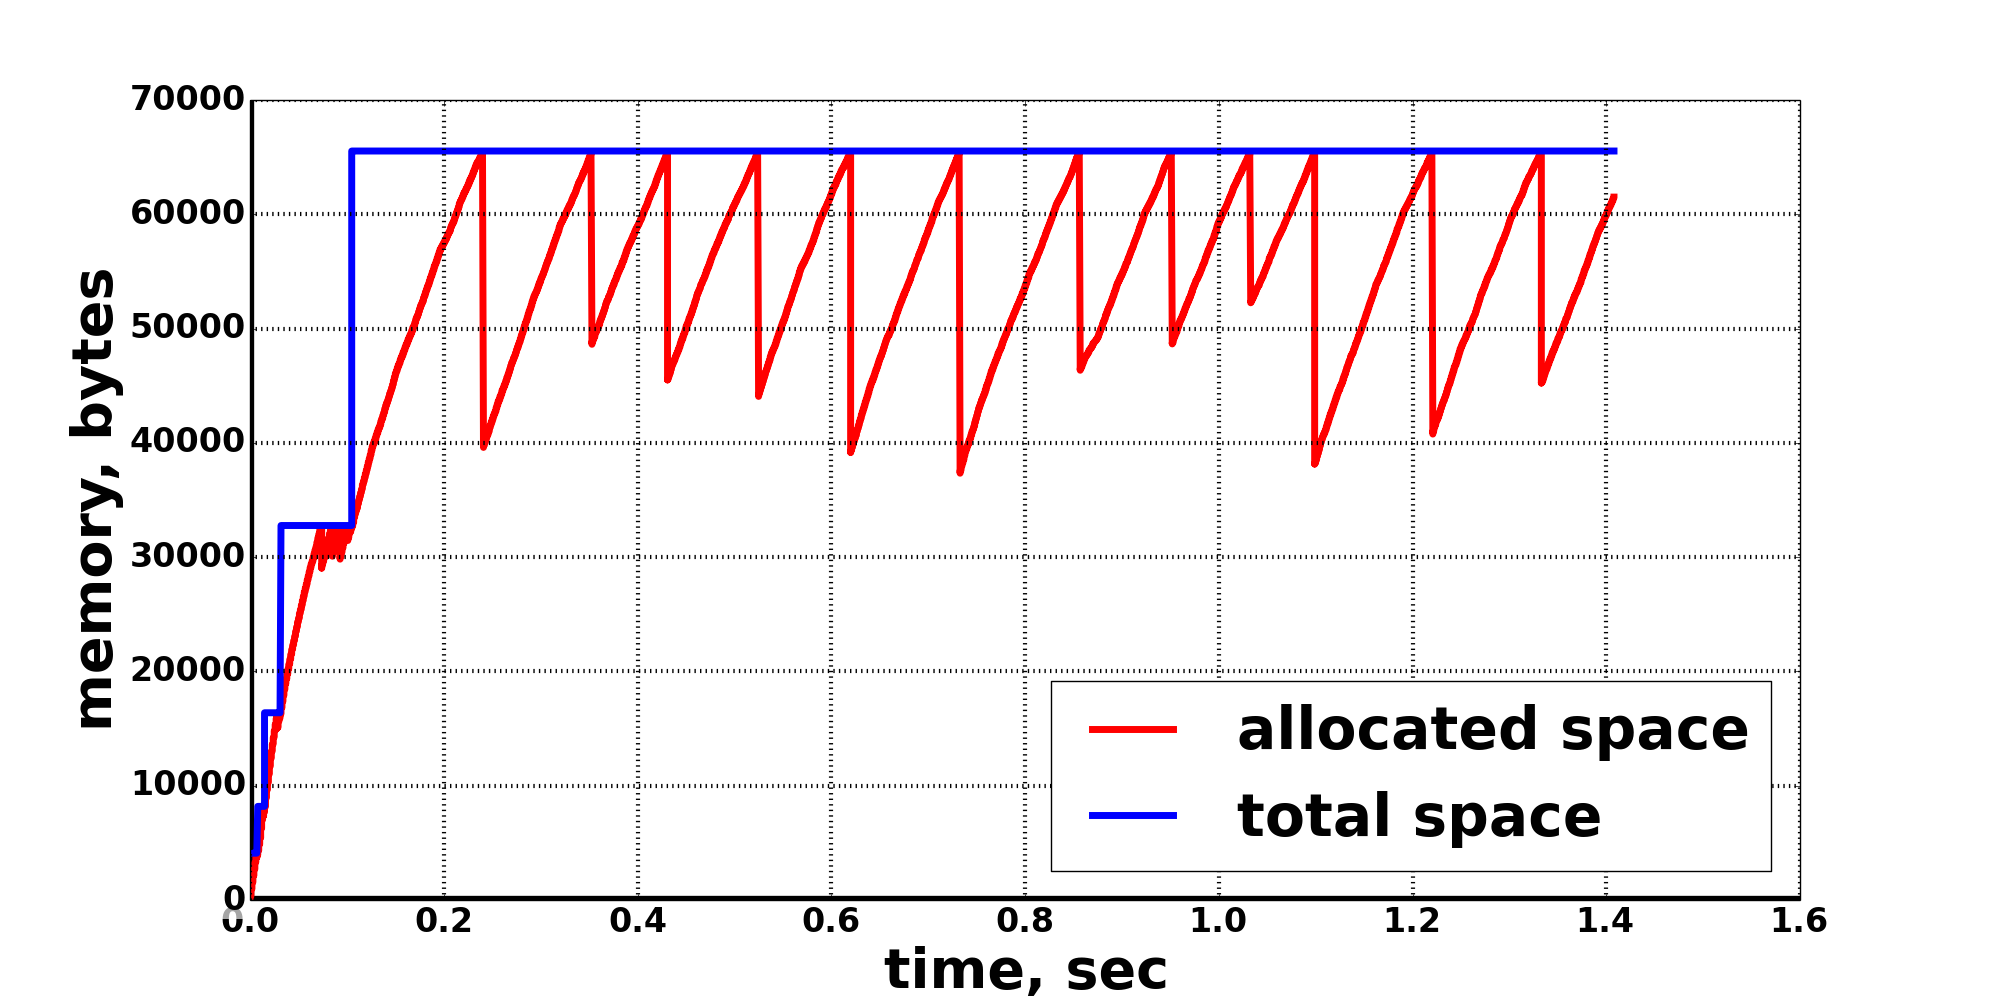
\includegraphics[width=1\linewidth]{Samofalov/parser-no-space.png}
\end{figure}
\section*{Заключение}
В результате данной работы был реализован подключаемый модуль для компилятора LLVM, обеспечивающий взаимосвязь между сборщиком мусора и компилятором языка на основе LLVM.  С использованием данного модуля был реализован mark-and-sweep сборщик мусора, работа которого была протестирована с помощью компилятора для языка OCaml. 

\begin{thebibliography}{99}
\bibitem{llvm} Chris Lattner.
LLVM: An Infrastructure for Multi-Stage Optimization.
Computer Science Dept., University of Illinois at Urbana-Champaign, 2002.

\bibitem{clang}
Dominic Fandrey. Clang/LLVM Maturity Report.
Computer Science Dept., University of Applied Sciences Karlsruhe, 2010.

\bibitem{lisp}
John McCarthy.
Recursive Functions of Symbolic Expressions and Their Computation by Machine //
Communications of the ACM, 1960.
\end{thebibliography}
